\subsection{Technische Umsetzung}

\subsubsection{Beschreibung der entwickelten Software}
Die Anwendung ist durch einen Login geschützt und das visuelle Interface responsive umgesetzt.
Die meiste Nutzung wird am Desktop stattfinden, daher ist die UI auch hauptsächlich darauf ausgelegt.
Das Design wird durch Nova vorgegeben und ist modern.
Die verwendeten Farben und das Logo wurden auf GRAW angepasst.

\newlineparagraph{Dashboard}
Nutzer bekommen einen Überblick über den Status von Stationen.
Aktuelle Flüge und deren Status sowie Messdaten werden in einer Tabelle und auf einer Karte dargestellt.
Die Anwendung prüft in kurzen Intervallen die Datenbank auf neue Daten und aktualisiert bei Bedarf automatisch die UI.

\newlineparagraph{Stations}
Stationen werden auf einer Karte und als Liste dargestellt.
Innerhalb einer Station werden das Dashboard dieser Station, sowie durchschnittliche Flugstatistiken dargestellt.
Außerdem können Stammdaten editiert, Nutzer zugeordnet und Flüge ausgewählt werden.

\newlineparagraph{Flights}
In einem Flug unterscheidet sich die Ansicht je nach Status.
Laufende Flüge zeigen den aktuellen Flugverlauf und aktuelle Daten.
Abgeschlossene Flüge zeigen Performancekriterien, thermodynamische Diagramme und Messwertdiagramme nach Zeit und Höhe.

\newlineparagraph{Users}
Systemadministratoren können neue Nutzer erstellen und deren Rolle festlegen.
Stationsadministratoren können für ihre verwalteten Stationen Nutzer erstellen.

\newpage

\newlineparagraph{API}
Für die Datenübertragung durch die native Anwendung GRAWMET wird eine RESTful (Representational State Transfer) HTTP Schnittstelle (\ref{fig:api}) bereitgestellt.
Der Zugriff wird mittels Basic Authentication (siehe~\cite{rfc7235}) abgesichert, die Kommunikation darf daher nur über HTTPS erfolgen, da Secrets sonst unverschlüsselt übertragen werden.
\begin{figure}[h!]
    \centering
    \caption{API}
    \label{fig:api}
    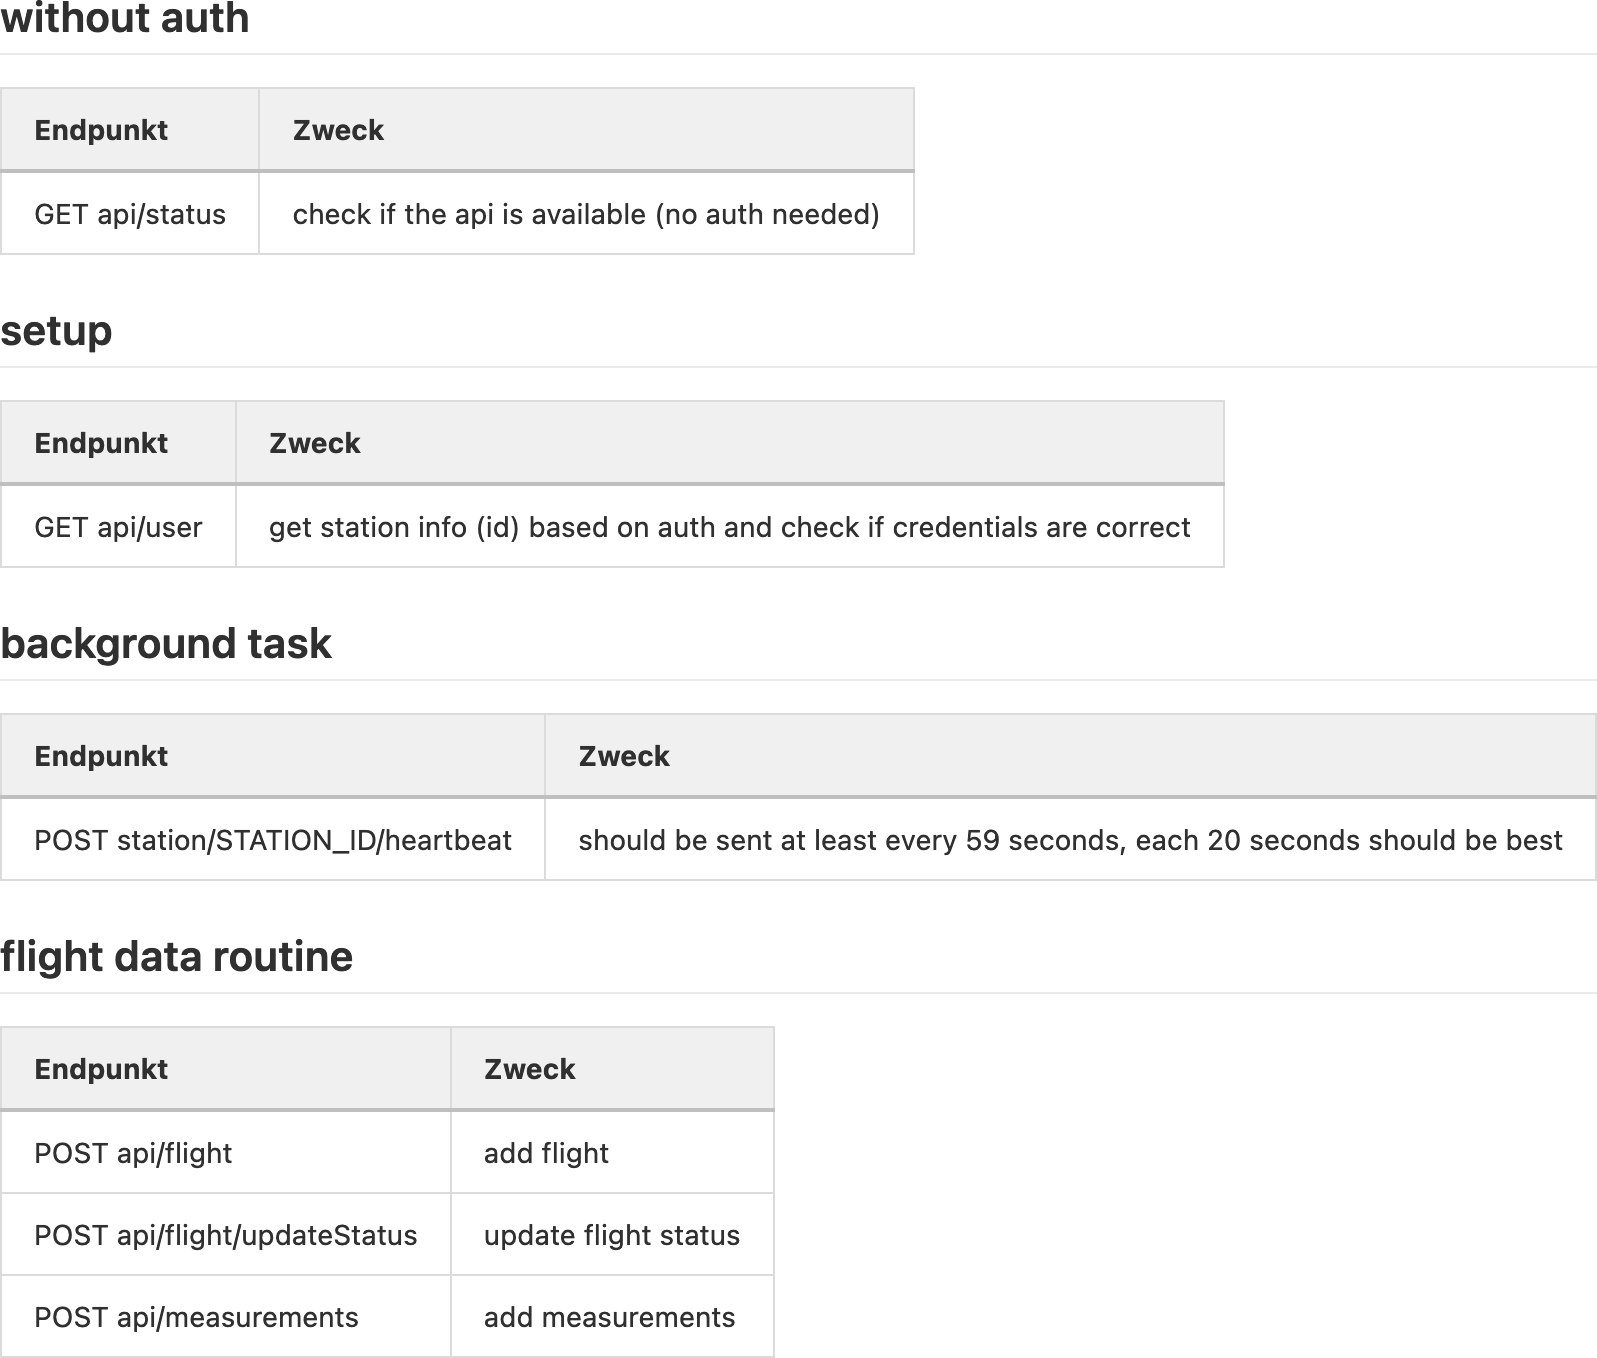
\includegraphics[scale=0.55]{assets/api}
\end{figure}

\newlineparagraph{Datenbankschema}
Für die zu speichernden Daten ist das folgende Schema (\ref{fig:db}) modelliert und, durch Laravel Migrations (siehe~\cite{laravel/migrations}), in Programmcode festgeschrieben.
\begin{figure}[h!]
    \centering
    \caption{Datenbankschema}
    \label{fig:db}
    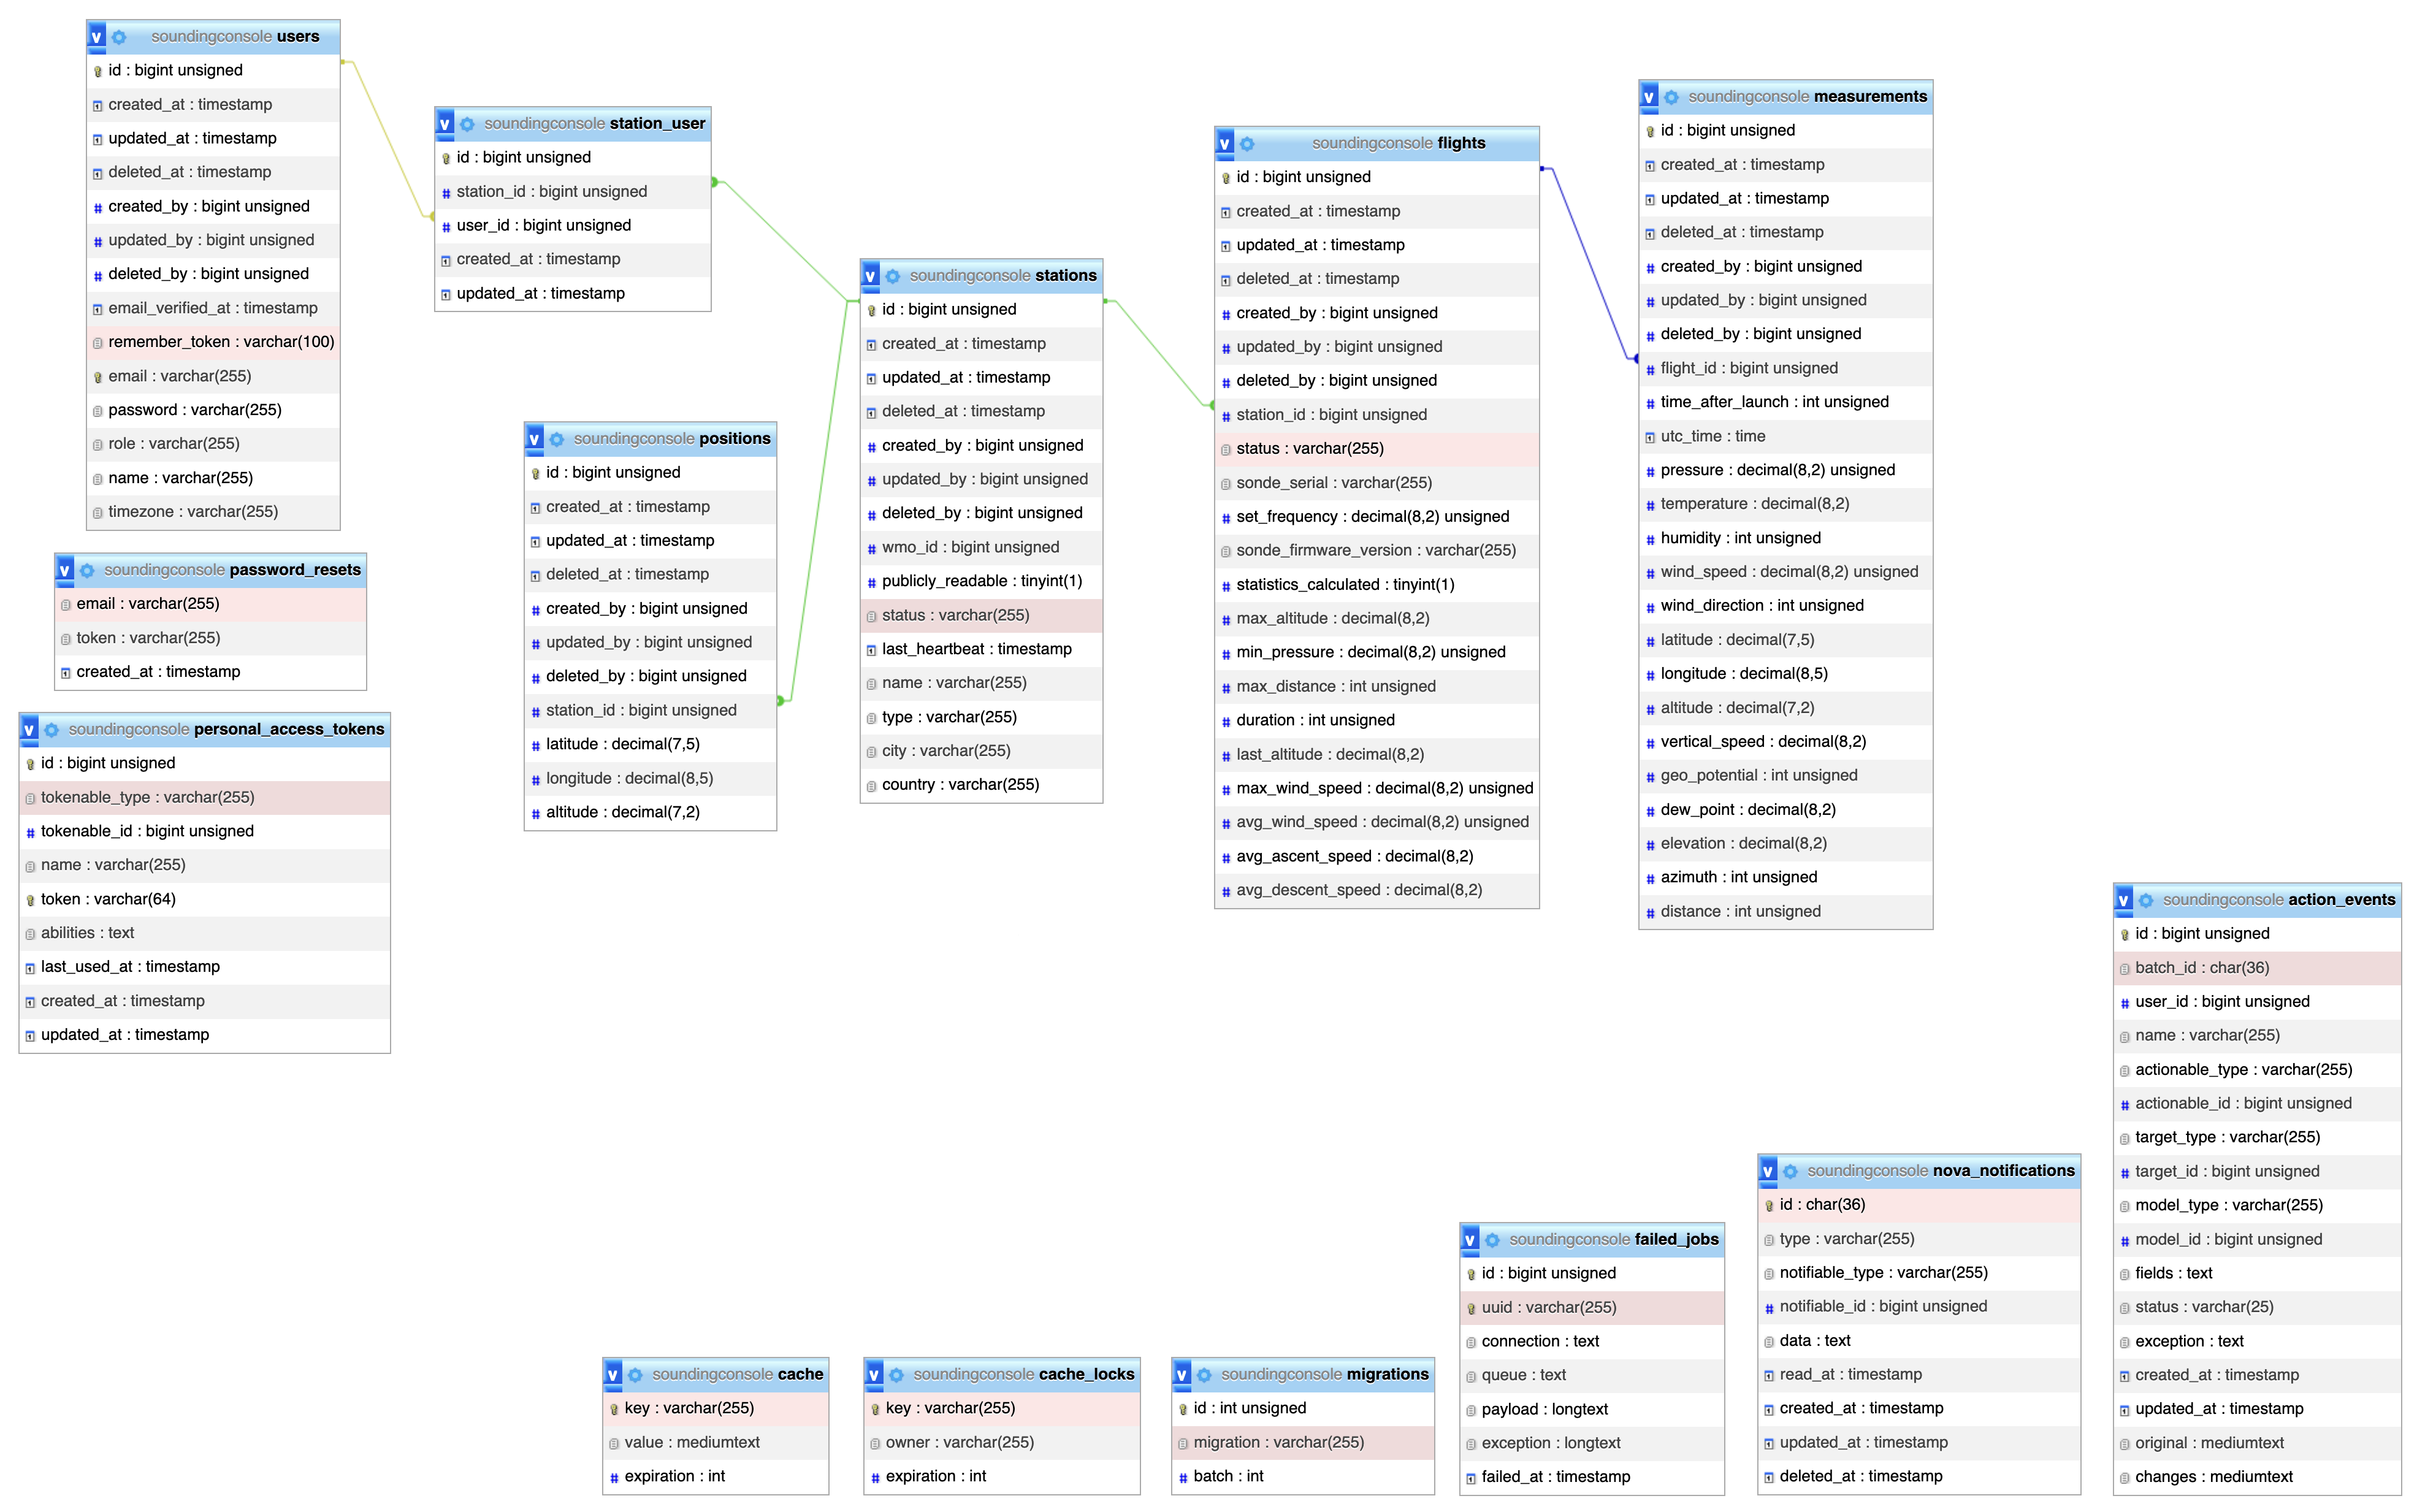
\includegraphics[scale=0.33,angle=90]{assets/db}
\end{figure}

\newpage

\subsubsection{Probleme und Lösungen}

\newlineparagraph{Thermodynamische Diagramme}
Im Projekt sondehub-tracker (\cite{sondehub-tracker}) gibt es ein fertiges Skew-T Diagramm.
Allerdings ist dies nur eine Projektkomponente und keine Library, und damit liegt die gleiche Problematik wie bei der Kartenkomponente vor.
Alternativ wurde bei einer weiteren Recherche jedoch die Library meteoJS gefunden.

Eine fehlende Dokumentation macht es leider notwendig, die vorhandenen Beispielimplementierungen zu analysieren und auf Basis dessen, die Komponente anzubinden.
Ebenfalls fehlt in dieser Library eine Legende, daher muss der Quellcode und die darin enthaltenen mathematischen Formeln analysiert werden, um die meteorologischen Messgrößen zu bestimmen.
Die Hürden sind überwunden und die Komponente ist funktionsfähig eingebunden.

\newlineparagraph{Kartenkomponente}
Ursprünglich sollte als Kartenkomponente das Projekt sondehub-tracker (\cite{sondehub-tracker}), bzw.\ Teile davon, eingebunden werden.
Bei genauerer Betrachtung fällt jedoch auf, dass dieses Projekt nicht als Library gebaut oder nutzbar ist.
Daher wurde es lediglich kurz analysiert und daraus die Entscheidung getroffen, die Library \enquote{Leaflet} zu nutzen.
Unter Einsatz dieser Library konnte eine interaktive Kartenkomponente entwickelt werden, welche Flüge, Stationen und Messwerte darstellt.

\newlineparagraph{Styling von Custom Components}
Im Projekt werden viele individuelle Komponenten verwendet, um die UX der Software in Nova möglichst stark zu optimieren.
Dafür werden teilweise Komponenten wie Tabellen und Überschriften benötigt, die Nova bereits selbst implementiert.
Nova bietet es offiziell nicht an, allerdings wurde eine Lösung gefunden, wie man alle Vue Single File Components von Nova auch in den individuellen Komponenten nutzen kann.
Es muss lediglich aus der individuellen Komponente heraus ein langer relativer Pfad, bis in das Nova-Quellverzeichnis, angegeben werden.
Danach können die Komponenten gebaut und genutzt werden.

Möglicherweise gibt es zukünftig Breaking Changes seitens Nova, da dieser Import eigentlich nicht vorgesehen ist.
Dies muss bei Updates beachtet und gegebenenfalls angepasst werden.

\newpage

\newlineparagraph{Infinite Loading Tables}
Laravel Nova unterstützt neben paginated Tabellen auch ein \enquote{Load more} Pattern.
Im Projekt wurde allerdings ein \enquote{Infinite Loading} Pattern priorisiert, um eine ähnliche UX wie die native Windows Anwendung zu bieten.
Da die Tabellenkomponente von Nova selbst nicht verändert werden kann, erweitert ein separates Skript, mittels Observer Pattern, die Komponente um diese Funktion.
Alternativ könnte eine individuelle Komponente gebaut werden, dies würde allerdings zu viele Basisfeatures von Nova entfernen.
Hier zeigt sich ein Problem in der Anpassbarkeit von Nova Anwendungen, im konkreten Fall allerdings ein lösbares.

\newlineparagraph{Tabellensortierung}
Nova erlaubt Nutzern die Sortierung von Tabellen nach einer Spalte und als Entwickler kann man auch den zugrundeliegenden Query bereits sortieren.
Allerdings kann keine Standardsortierung nach einer Spalte konfiguriert werden.
Diese Einschränkung bei Messwerttabellen muss fürs Erste so hingenommen werden.
Bei stärker priorisiertem Bedarf, kann die Standardtabelle, durch eine individuelle Komponente, ausgetauscht werden.

\newlineparagraph{Verlassene Library}
Es gibt einen Fehler in der JSON Schema PHP Library, dieser wurde beim manuellen Testen der entwickelten API mit unterschiedlichen Werten gefunden.
Für die Problematik wurde folgender Issue erstellt: \url{https://github.com/opis/json-schema/issues/123}

Die Aktivität im Repository lässt allerdings vermuten, dass dieses Projekt aufgegeben ist.
Daher wurde vorerst die fehlerhafte \enquote{multipleOf} Validierung entfernt.
Vermutlich muss zukünftig eine andere Bibliothek gefunden werden, welche die notwendigen JSON Schema Regeln korrekt implementiert.
